\section{Visual Exploration of Query Results}\label{sec:otherFunctions}
In addition to the feature and pattern detection methods described in Sections~\ref{sec:automaticExtraction} and \ref{sec:visualQuery}, TimeTubesX includes powerful visual comparison and annotation features for further analysis of blazar data.

%the present analysis functions for extracting features in a synergetic way,
%we introduce several auxiliary functions into TimeTubesX.

\subsection{Visual Comparison of Query Results}
An essential feature for analysis of blazar datasets is the user's ability to compare query results---not just within a single query but also to previous query results. 
For example, when users find that a specific feature frequently appears in a certain time period,
they might want to investigate whether any other features also frequently appear in the same time period.
Therefore, TimeTubesX can juxtapose the results of different queries
by loading query results that were previously saved as a JSON file.
%
%They can store the query information with the annotation function, but extraction results are automatically overwritten every time they run a new query.
% Furthermore, users can save and load query results to and from disk, as a JSON file, to allow comparisons even between different sessions and users.
%, users can export extraction results as a JSON file and import the file.
When importing a file, the stored results are mapped to a new timeline that is arranged as a juxtaposed view below the original timeline.
%in different colors from the current extraction results.
Hovering over marks on the timeline allows users to see detailed information about specific results.
Additionally, users can re-use or review the settings of the previous query, such as the selected time period or the variables assigned to the sketch pad (see Fig.~\ref{fig:UIFeatureExtraction}~(F)).
%If needed, they can reuse the previous query.

% \subsection{Annotations of time steps, queries, and query results}
\subsection{Annotations of Queries and Query Results}
%
To enable efficient collaboration between astronomers and to facilitate keeping track of analyses between different sessions, TimeTubesX supports detailed annotations for query results.
% Annotations allow users to document their analysis process and to share their results with others.
% queries, query results, and time spans of interest.
%
%The users can annotate extracted results. 
Users can access any annotations even after exiting and restarting the application because annotations are stored in the local storage of the web browser. 
To share annotations with other users, annotations can be exported as a single JSON file. 
%The users are allowed to export the annotations as a JSON file, which will make it easy to share insights among the colleagues.
The system stores the annotation's time stamp, username, comment, and dataset, as well as detailed information about the query and query results.
Users can see all of their annotations in a table view or a single annotation by clicking on a marker with the selected label color in the TimeTubes and scatterplots views.
They can also re-use any query saved in an annotation by simply clicking on it. %just by selecting an annotation.

Annotations help users highlight interesting extraction results.
% of the feature and pattern detection.
%
% This is especially important to iteratively refine queries, to exclude those time intervals that do not reflect the user's intentions.
%
%because the feature extraction of TimeTubesX presents candidates for characteristic blazar behaviors or time intervals resembling the input pattern, but time intervals which do not reflect the users' intentions enough might also be included.
Annotating time intervals of interest not only triggers deeper inspection of a specific period 
but also possibly facilitates the discovery of new features such as periodic patterns.






% \begin{figure}[tb]
%     \centering
%     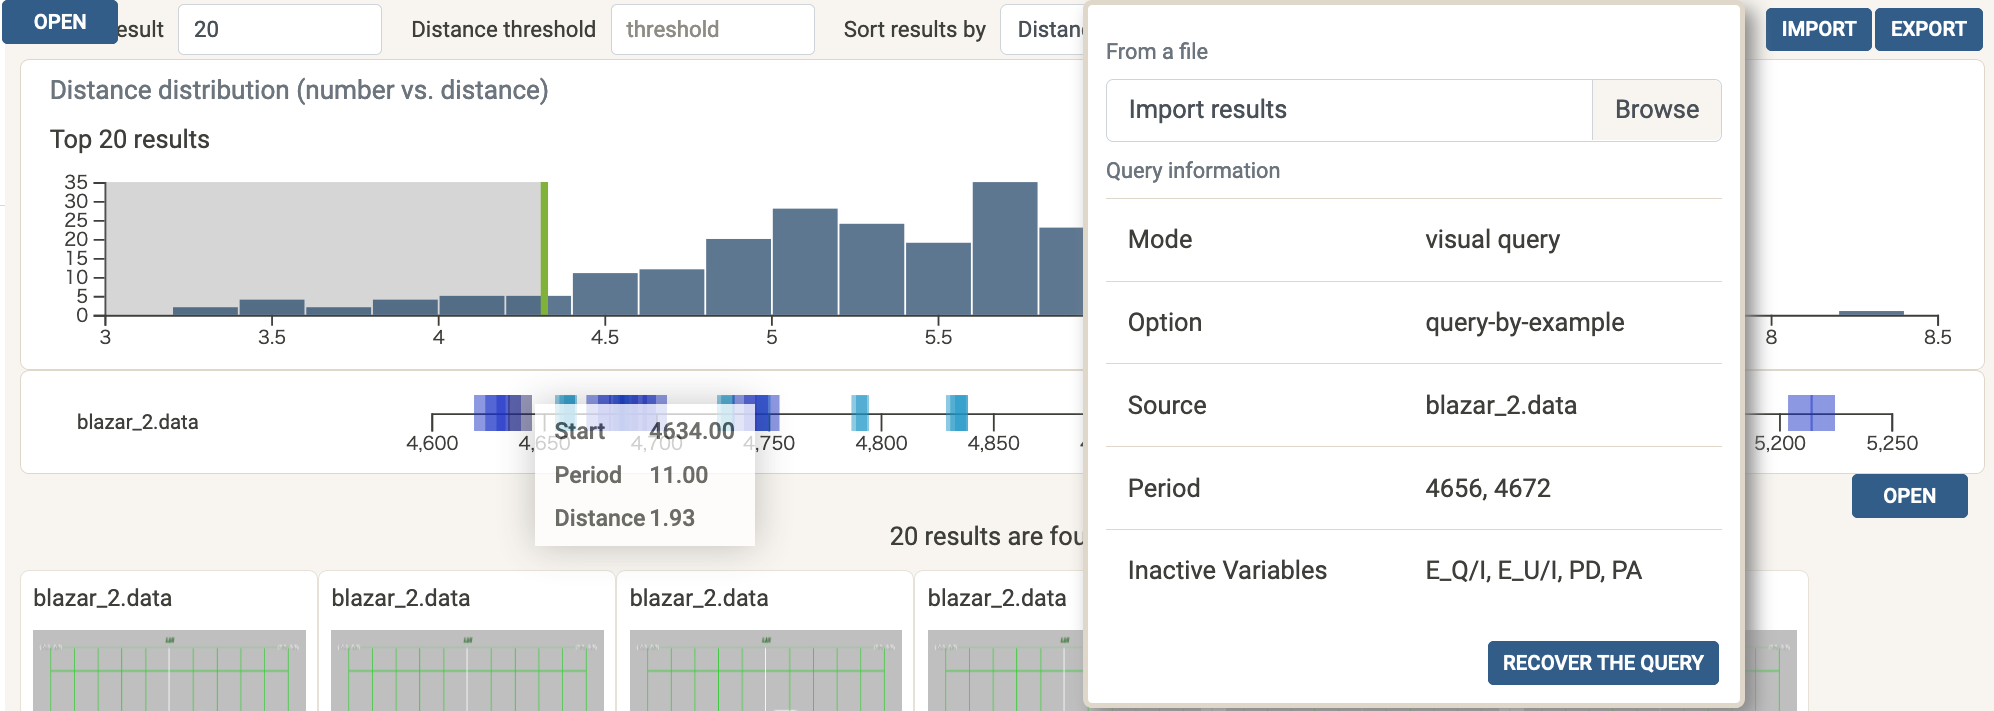
\includegraphics[width=.99\linewidth]{vgtc_journal_latex/figures/resultComparison.png}
%     \caption{Comparing the current extraction results with the previous ones. 
%         Light blue plots indicate the current extraction results, 
%         while dark blue plots do the previous ones.}
%     \label{fig:resultsComparison}
% \end{figure}
% \subsection{Implementation}\label{sec:Implementation}
% TimeTubesX is a browser-based application written in HTML and Javascript.
% We use React.js to build user interfaces and flux.js to manage the application state.
% We also utilize standard libraries such as D3.js~\cite{d3_framework} and paper.js~\cite{paper_framework}.
% TimeTubesX is open-source and running system can be found at \url{https://timetubes.herokuapp.com/}.